\chapter{General Discussion}\thumbforchapter
\newpage

\begin{shadequote}[c]{George Box}
All models are wrong, but some are useful.
\end{shadequote}

\section{The phylotypic stage}

While historically, the phylotypic stage has predominantly been examined and described through qualitative methods, the 21\textsuperscript{st} century started a paradigm shift towards a more quantitative and data-driven approach to understanding this phenomenon\cite{Chan2021}. The first notable quantitative investigation into the phylotypic stage was done by Bininda-Emonds \textit{et al.}, where they calculated temporal conservation as the order in which morphological embryonic features appear in vertebrates. However, it wasn't until the early 2010s that the field truly embraced quantitative methodologies with the simultaneous publication of two groundbreaking studies in Nature\cite{Kalinka2010, DomazetLoso2010}. In these works, Domazet-Lošo \textit{et al.} investigated the average developmental age of transcripts in \textit{D. rerio} and \textit{D. melanogaster}, whilst at the same time, Kalinka \textit{et al.} explored the temporal transcriptome similarities across different \textit{Drosophila} species. These molecular studies opened a new line of research to the quantitative basis of the phylotypic stage. Quantitative support for the phylotypic stage got stronger and stronger with each new study. So strong, that we quickly forget all the nonconforming studies.

The transcriptome age index (TAI), that Domazet-Lošo \textit{et al.} proposed, is the average transcript's evolutionary age calculated over time. The evolutionary age is defined as the number of taxonomic branches the gene dates back to. The idea of the TAI is that a temporal change is informative of more or less conservation. However, an independent re-analysis by Piasecka \textit{et al.} showed that due to major differences in transcript levels per gene, only a small subset of genes significantly influence the TAI\cite{Piasecka2013}. Log transforming the data, which is a standard processing step for this type of data, completely invalidates the results of the original study. One would ideally hope that this dependence of the results on transforming the data disqualifies the methodology, but the opposite appears to be true. The study that introduces the TAI is cited 88 times in the period between 2010-2013, and 359 times since the publication of Piasecka \textit{et al.} (years 2014-2023). It turns out that you can now analyze the data with and without transformation, and keep the results that confirm your preferred hypothesis. An example of this is the study of Spiralian development by Wu \textit{et al.}\cite{Wu2019}, where they calculate the TAI on untransformed data for \textit{Crassostrea gigas}, \textit{Haliotis discus hannai} and \textit{Perinereis aibuhitensis}. Based on their results they claim that all three species show an inverse hourglass. The supplementary files, however, contain the TAI of \textit{Crassostrea gigas} after square root transformation, where the pattern changes from an inverse hourglass into a funnel. The  The authors practically ignore this result, and only conclude that at least it is not an hourglass-like pattern. Unrelated but worth mentioning is that the TAI of \textit{Perinereis aibuhitensis} appears to be random noise. Where this study should be taken with a grain of salt, three influential evolutionary-developmental biologists (Pavel Tomanczak, Denis Duboule, and Andreas Hejnol) interact with each other on Twitter discussing this study and the implications for the universality of the hourglass model. Andreas Hejnol has authored two criticisms of previous studies that claimed the phylotypic stage to be universal\cite{Dunn2018,hejnol2016}.

The work of Barbara Piasecka, where she showed that the pattern of the TAI is caused by a subset of all genes was led by Marc Robinson-Rechavi. The main work of this study was not about the TAI, but about using a multitude of different metrics to estimate temporal evolutionary conservation. Their conclusion is that different metrics give different results. This is important, as perhaps (temporal) conservation is not that easy to measure, and/or depends on the methodology used. Marc Robinson-Rechavi in his later career, however, seems to have forgotten his conclusion and makes strong claims about the ortholog conjecture\cite{KryuchkovaMostacci2016} (methodological problems with this study were found\cite{Dunn2018}), and the hourglass model of conservation\cite{Liu2020,Liu2021,marletaz2018} (two of which I show have methodological problems in chapter XXX). 

In 2003 Bininda-Emonds \textit{et al.} showed an unexpected inverse hourglass on morphological rankings\cite{OlafRP2003}. Seventeen years later, Gerardo A. Cordero \textit{et al.} did a similar analysis of morphological timings across more species and morphological features\cite{Cordero2020}. To my knowledge, these are the only quantitative analyses of morphological characteristics with respect to the phylotypic stage. Cordero \textit{et al.}, surprisingly, find the exact opposite of Bininda-Emonds \textit{et al.}; namely an hourglass pattern. Surprisingly, Cordero \textit{et al.} only commented that the difference between these two studies \textit{could} be caused by a difference in morphological characteristics, methodology, and species used. The main analysis of Bininda-Emonds \textit{et al.} is a mean-variance plot, something that takes 5 minutes to make.

The inverse hourglass model between phyla, proposed Levin \textit{et al.}, as a between phyla phenomenon\cite{Levin2016}. This study has been rightfully criticized by Casey Dunn and Andreas Hejnol for the lack of a within-phylum comparison\cite{hejnol2016}, and improper statistics\cite{Dunn2018}. It has been seven years since this issue has been raised, and still has not been adressed by Levin \textit{et al.}. It is relatively little work for their major claim of a universal phylotypic stage of high similarity within phyla, but low similarity between phyla. Perhaps even more confusing, when a different group of evo-devo biologists investigated the transcriptome similarity between deuterostomes and the chordate amphioxus, which is a between phyla comparison, they show an hourglass-like pattern\cite{PerezPosada2022}. This is in direct contradiction to the inverse hourglass model of Levin \textit{et al}. Why don't they comment on this? They must have noticed.

\begin{figure}[H]
    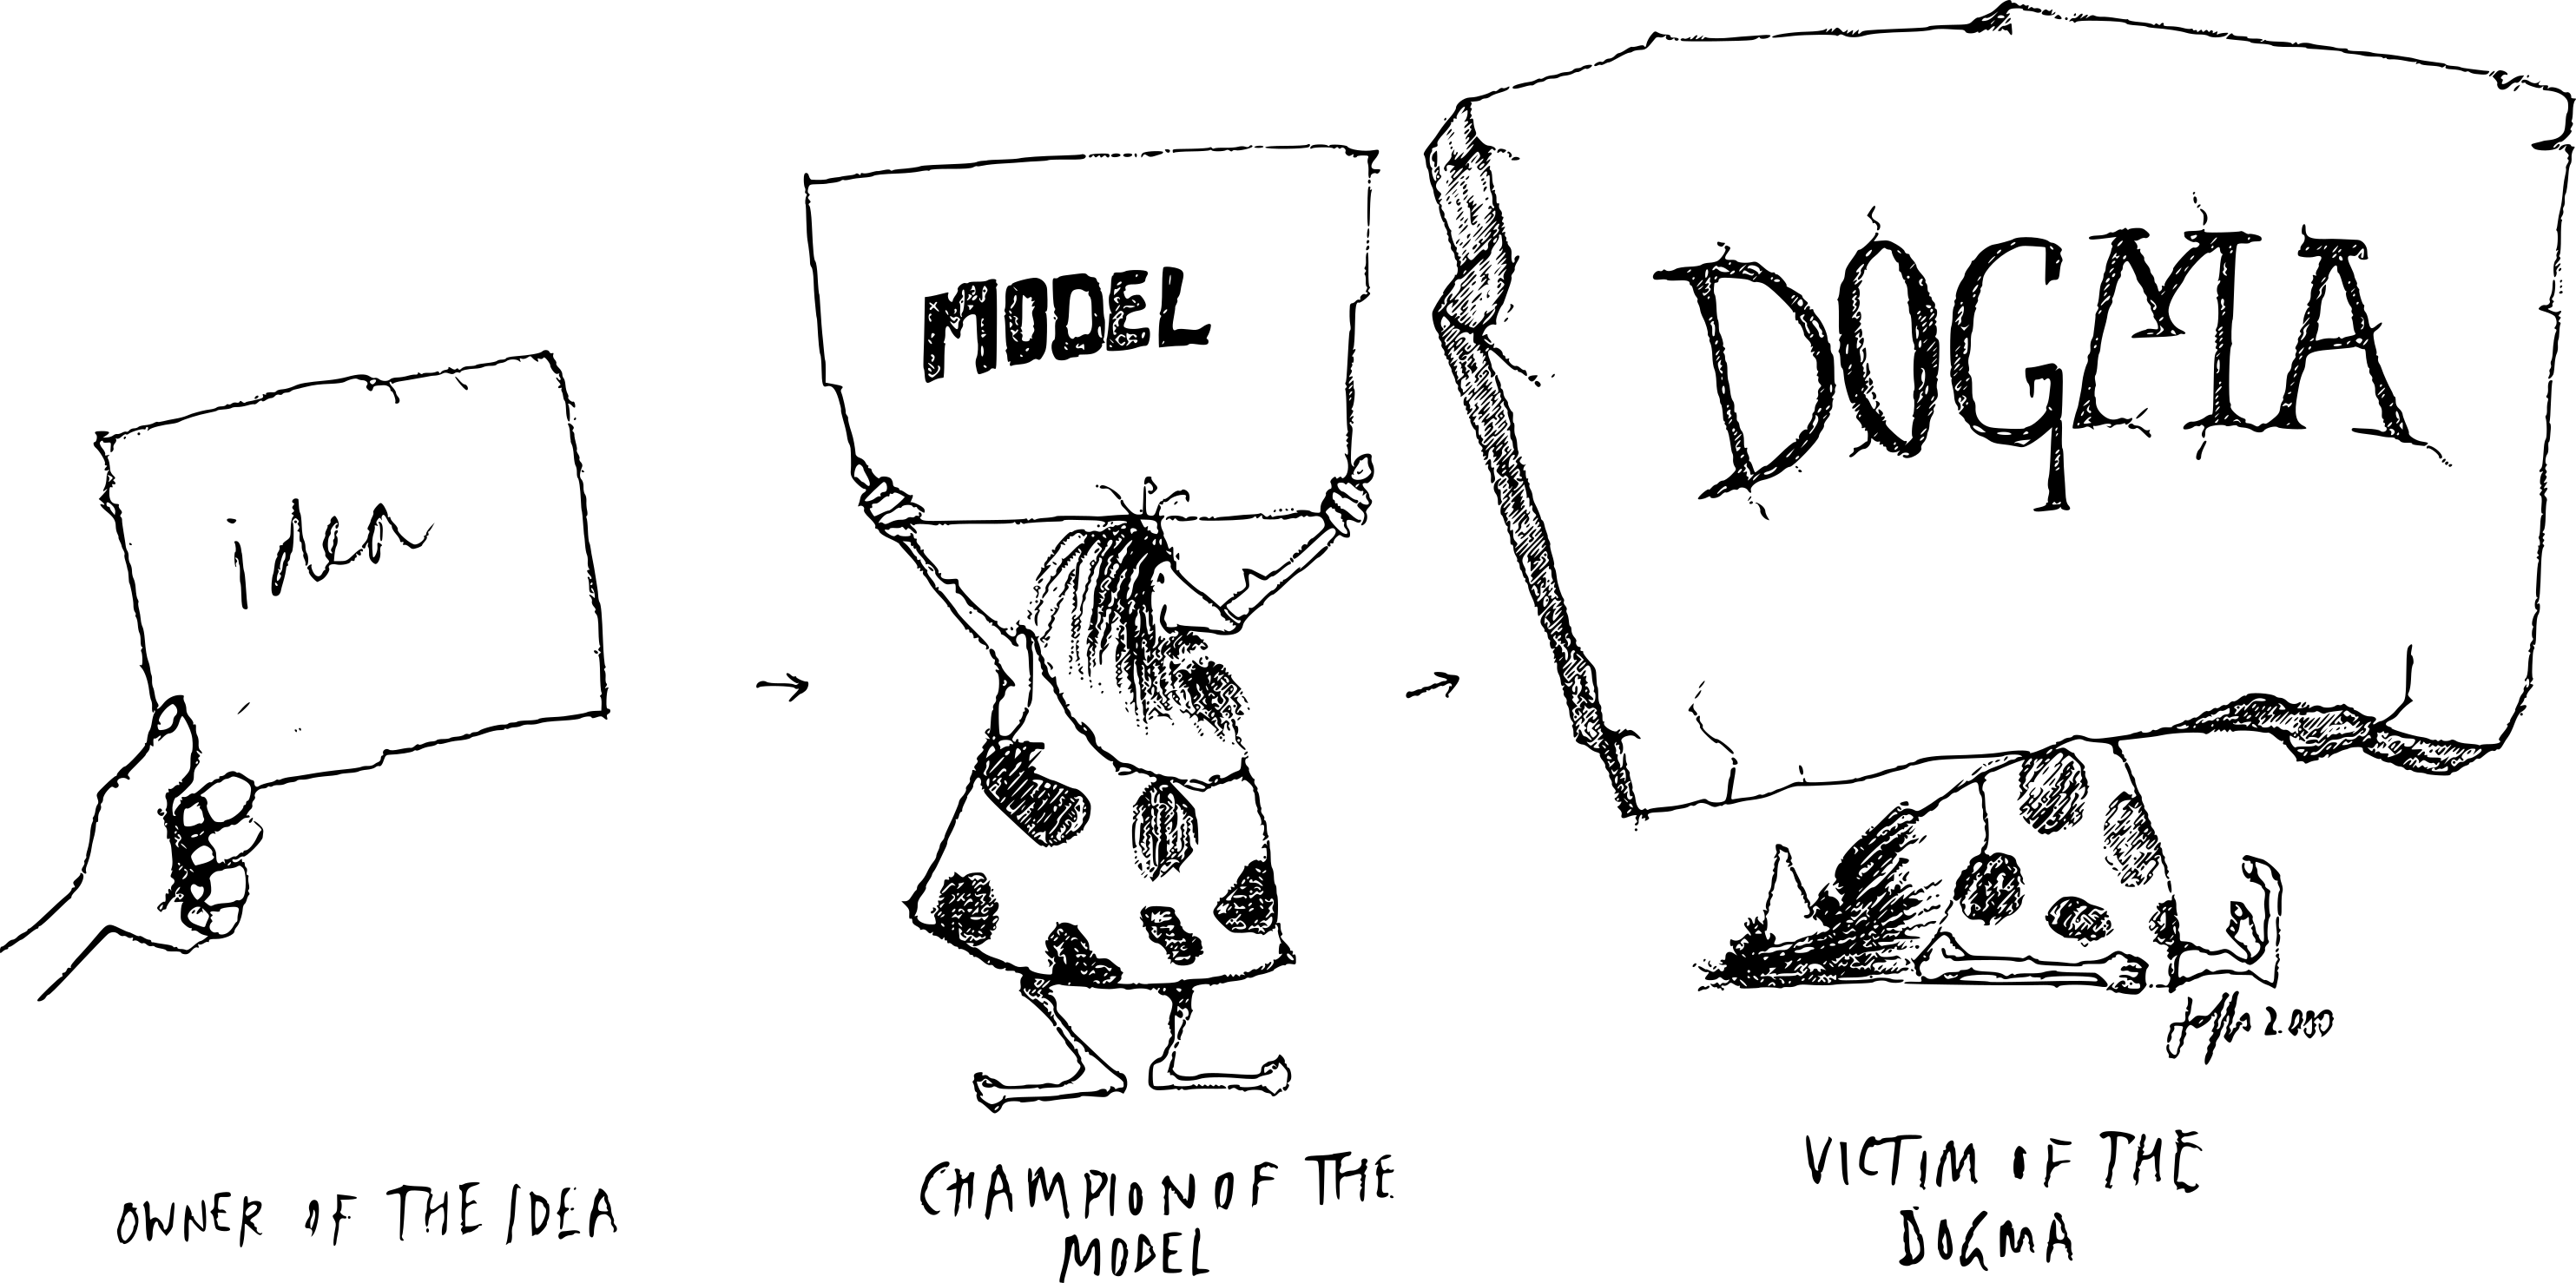
\includegraphics[width=\linewidth]{ch.discussion/imgs/dogma.png}
    \caption{\textbf{The phylotypic stage as a dogma} \cite{Caveman2000}.}
    \label{fig:dogma}
\end{figure}

Yoav Mayshar \textit{et al.} studied the phylotypic stage and the hourglass model from a single-cell point of view\cite{Mayshar2023}. They compare the proportions of different cell types between developing rabbit and mouse embryos. I show in chapter X that the time series of the mouse and rabbit are both discontinuous, and thus the temporal correlations between rabbit and mouse are an effect of this. If anything, the discontinuous pattern in cell type proportions can be interpreted as a mid-developmental transition and as an inverse hourglass. But somehow, Mayshar \textit{et al.} interpret this pattern exactly opposite, and claim that this is an hourglass. How was this not caught by the reviewers of Cell, one of the most prestigious journals? When I asked Y. Mayshar on Twitter if the pattern is not actually the inverse of what they claim, he comments with \say{this basically shows convergence of frequencies of cell states at \~e7.5-e8, preceding what would be normally considered as the phylotypic stage, though this is pretty vaguely defined...}. 

There seems to be a certain level of apathy to each other's work when studying the phylotypic stage. Nearly all studies in this field contain obvious methodological problems, but they are treated as unimportant as long as these studies confirm your own prior beliefs. In chapter X and Y I show and discuss newly discovered problems with comparative approaches. I fear that highlighting these problems won't actually matter for the field, as people will still believe their pet theories, and there will always be some methodology that "confirms" it. For example, a colleague of my department told me that even though I show that most methodologies are wrong, the phylotypic stage still obviously exists. What obvious information am I missing?

Based on my own re-analyses, it seems like most methodologies actually support the null model, where no point of higher/lower temporal conservation exists. The hourglass-like pattern based on transcriptome data (zebrafish vs xenopus) can be explained by within-species correspondence alone, both the transcriptomic inverse hourglass as the morphological inverse hourglass can be recreated with random data with no temporal conservation, and the wrongly annotated hourglass of cell type proportions is caused by discontinuous temporal sampling. Only the drosophila enhancer conservation re-analysis gives a (different) point of maximum conservation, except that I think the methodology is not correct anyways. It could be that this means that there just isn't any temporal conservation. Or that the noise in these models is bigger than the signal. Perhaps the temporal conservation effects aren't that large, or the variation between species and methodologies is many times larger? Some things are just extremely difficult to measure observationally. Without experimental studies .

Moreover, there is no consensus about what is actually expected to be conserved. The original observation that embryos, perhaps, look more like each other at certain points in development than at other times, says nothing about the molecular basis for this. It has been quantitatively studied on the basis of embryonic lethality, morphology, DNA sequence conservation and activation order, cell type proportion, and whole-transcriptome similarity, with differing results. 

Scientists came up with the hypotheses of taxonomic phyla and the phylotypic stage. But somehow along the way, these hypotheses are now taken to be true, and require a molecular explanation. Just as that phyla are defined as a group of animals with the same body plan, and the body plan is defined as the shared body plan of all animals of the same phyla\cite{BUDD2000}. The phylotypic stage on the other hand is often defined as the developmental stage with the most similarity, but simultaneously the point of most similarity is then claimed to be the phylotypic stage\cite{Kalinka2010}. Morphologically and historically the pharyngula stage\cite{https://doi.org/10.1093/icb/21.2.391}, early somite embryos\cite{ https://doi.org/10.1046/j.1420-9101.1993.6030457.x}, and the tail bud stage \cite{Slack1993} have all been proposed as the vertebrate phylotypic stage. The definition of the phylotypic stage in molecular studies in turn depends on which stage shows the highest conservation, for instance the molecular phylotypic stage as the pharyngula \cite{Irie2011} or the early somite embryo \cite{DomazetLoso2010}. Nonconforming results are not seen as disproving these hypotheses, but are either ignored or seen as delimiters about where conservation acts. As such the hypothesis of a phylotypic stage is not only wrong, it is also not useful.

\section{scepia: gene regulatory networks}

Almost all gene regulatory approaches are context specific. But in the end a single set of instructions (DNA) for all contexts.

% \section{Do I regret seq2science?}

\section{The future of biology}

\subsection{Computational}

\subsection{lack of unified data encode like stuff}

For seq2science paper we tried paper X, Y, Z. DIFFICULT to get similar results.     

% No similarity between replicates:
% https://www.nature.com/articles/s41467-019-12687-4
% 
%  - drosophila sample missing and two other samples swapped
%  - inverse hourglass time orientation has negative values

NCBI sra is growing exponentially \cite{srawebsite}, but it is poorlymaintained.? It is an absolute pain to download from NCBI sra, hence sra-explorer, pysradb, fetchfastq, nf-core/fetchngs, and seq2science download-fastq workflow. Even more painful is that samples are submitted in non-standardized format. Need for MetaSRA and ALE. Works poorly, and is not necessary. Just properly add data. ENCOED is really nice

Single cell datasets often useless as only two out of three reads submitted. Single cell data is increasingly large.

Searat vs scanpy major differences in their log fold change calculation. How is this allowed?

\subsection{Open Science}



\subsection{Too much descriptive, not enough understanding}

Early adopters have been overwhelmed by the size of the data, lack of analytical tools, but mostly the number of different cell types generating a flurry of research articles with titles like "single cell sequencing in tissue X reveals heterogeneity".  

\subsection{Move away from mRNA}

mRNA and protein relation.
The correlation between protein expression and mRNA expression seems high (0.87) measured across cell types. However, genes with high protein expression generally have high mRNA expression. So it is easy to get high prediction. If you want to predict a single gene you get correlation of 0.41. Simpson's paradox! 
https://www.nature.com/articles/nature23293

https://www.biorxiv.org/content/10.1101/2023.05.23.541948v1

cool work of michael levine on xenobots

% https://twitter.com/nimwegenlab/status/1671923176626847744?s=12&t=oyB_faiBr8aHqHcjXZE50A

\begin{figure}[H]
    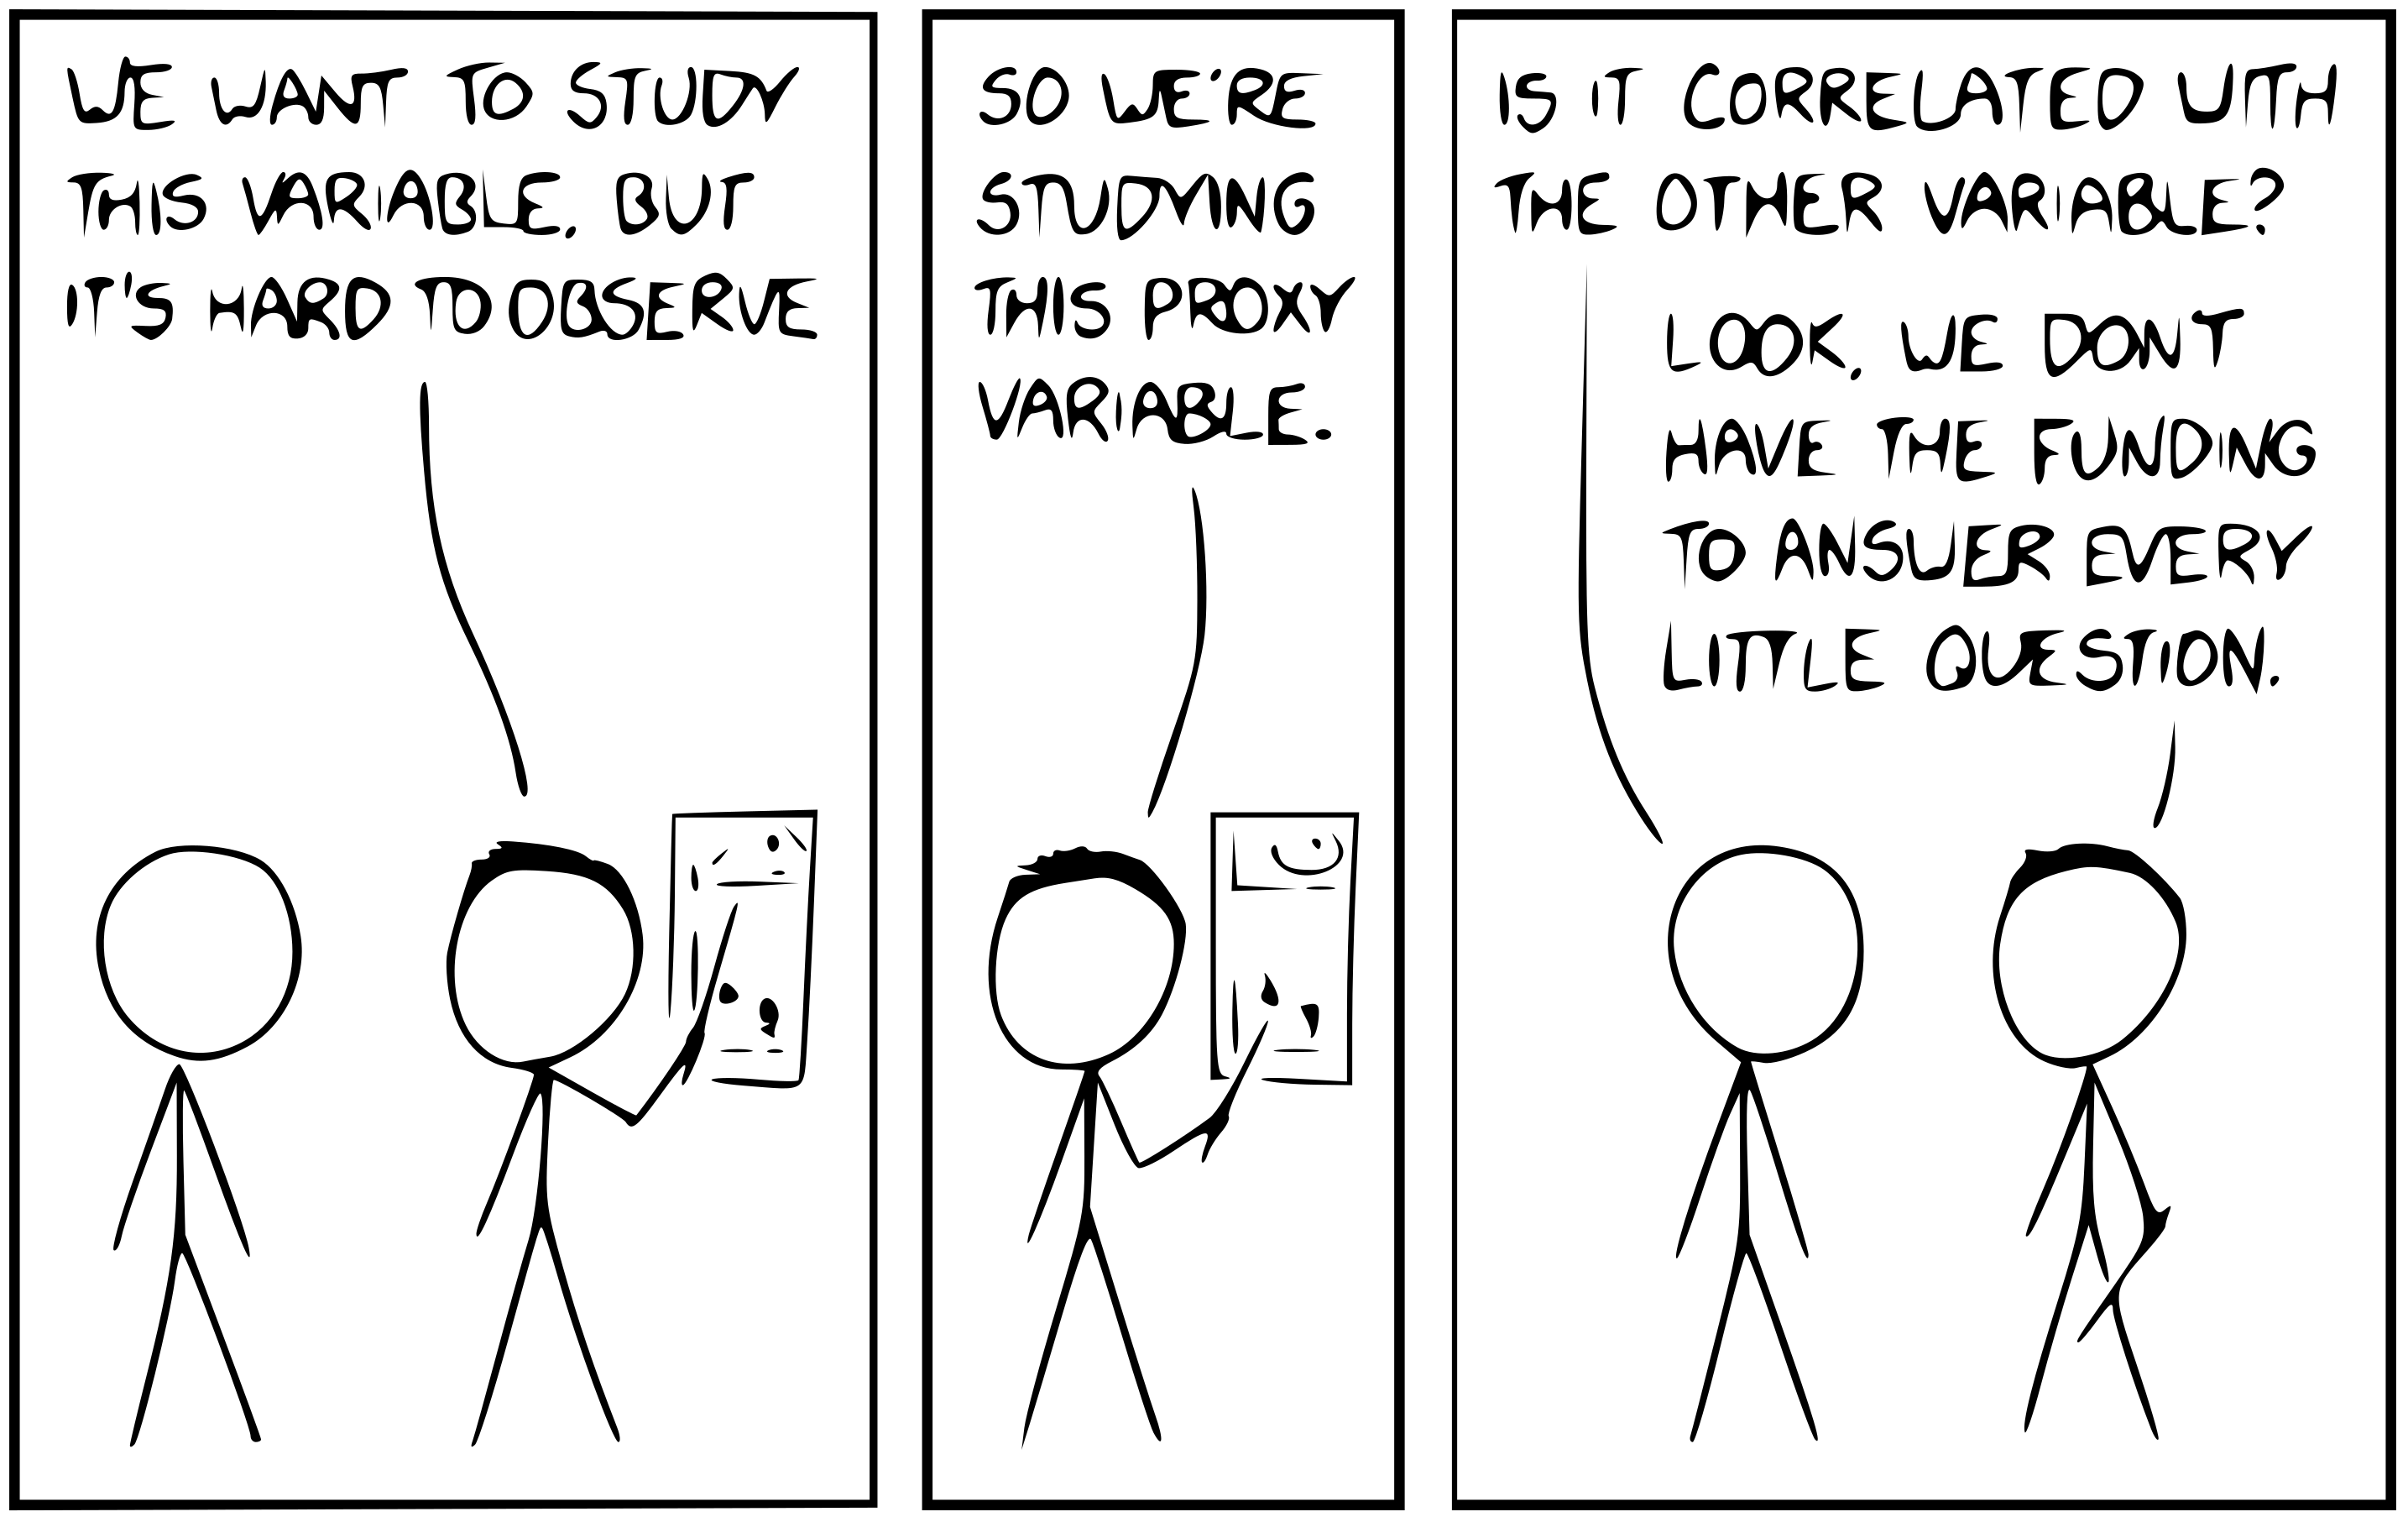
\includegraphics[width=\linewidth]{ch.discussion/imgs/xkcd.png}
    \caption{\textbf{xkcd}. URL: https://xkcd.com/2652}
    \label{fig:xkcd}
\end{figure}

% \subsection{Stop blaming "the incentives"}

% incentives: https://www.talyarkoni.org/blog/2018/10/02/no-its-not-the-incentives-its-you/

\subsection{Self-correcting}

e.g. wild growth covid papers

papers keep on being cited after retraction or criticism. Number one paper of percentage of genome is functional gives highly criticized ENCODE paper.

highlight cancer microbiome paper: https://www.nature.com/articles/s41586-020-2095-1. And the negative result : https://www.biorxiv.org/content/10.1101/2023.07.28.550993v1.full.pdf

comparison of mouse vs human transcriptome: https://www.pnas.org/doi/full/10.1073/pnas.1413624111 and the re-analysis that they were wrong: https://f1000research.com/articles/4-121/v1

ENCODE claiming 80\% biochemical and criticism on it. When googling first result is ENCODE (I think)

Our golden standard is actual clinical trials! Our methods don't seem to work so well..?
https://www.ncbi.nlm.nih.gov/pmc/articles/PMC6409418/
https://journals.plos.org/plosmedicine/article?id=10.1371/journal.pmed.0020124

% Biology is messy, but that does not mean computational biology has to be.
